\chapter{Web Threats}
\section{What is a Web Threat}

Put simply, a web threat is any malicious attack that uses the Internet as its main method of distribution, meaning that the types of web threats is wide and varied.  Web threats can be broken up into two main cateogires referred to as push or pull.  Pull based threats are attacks that can affect any visitor to the website or service while push based attacks use luring techniques to get a user to fall victim to the attack.  The main motivator behind these attacks is for the pursuit of confidential information and it is becoming more and more commonplace to hear about large scale data breaches.  While it is difficult to track all of the monetary gain from these activities due to the underground nature there are some instances of millions of dollars being extorted from large businesses.  As the number of users and the complexity of the devices attached to these networks increases so to it does the exploitability.  Common web attacks can range from simple phishing emails, to malicious email attachments to malicious code injection directly into a vulnerable website.

Attackers will vary their methods and tools often creating a situation where the attacker is always a step ahead of the preventation systems due to the unlimited number of possibilities.  This leads to the conclusion that conventional approaches grand-fathered in from other security sectors like virus scanning are not adequate for web threat detection.  There are two main reasons for this: first off the attacks are so varied in their approaches and transportation techniques that collecting samples to produce signatures for detection is not enough, the second reason is that unlike conventional viruses web attacks are designed to go under the radar instead of spreading as fast as possible.  Web servers are required to be publically open to the world unlike traditional desktop computers which typically have all ports closed, this opens up the problem of accepting information from unknown parties.  Therefore, modern solutions employ a much more layed approach using conventional detection methods along with reputation systems.
% Trend micro whitepaper ^^ %
% Forward reference chapter 3

\begin{figure}
	\label{fig:osithreats}
	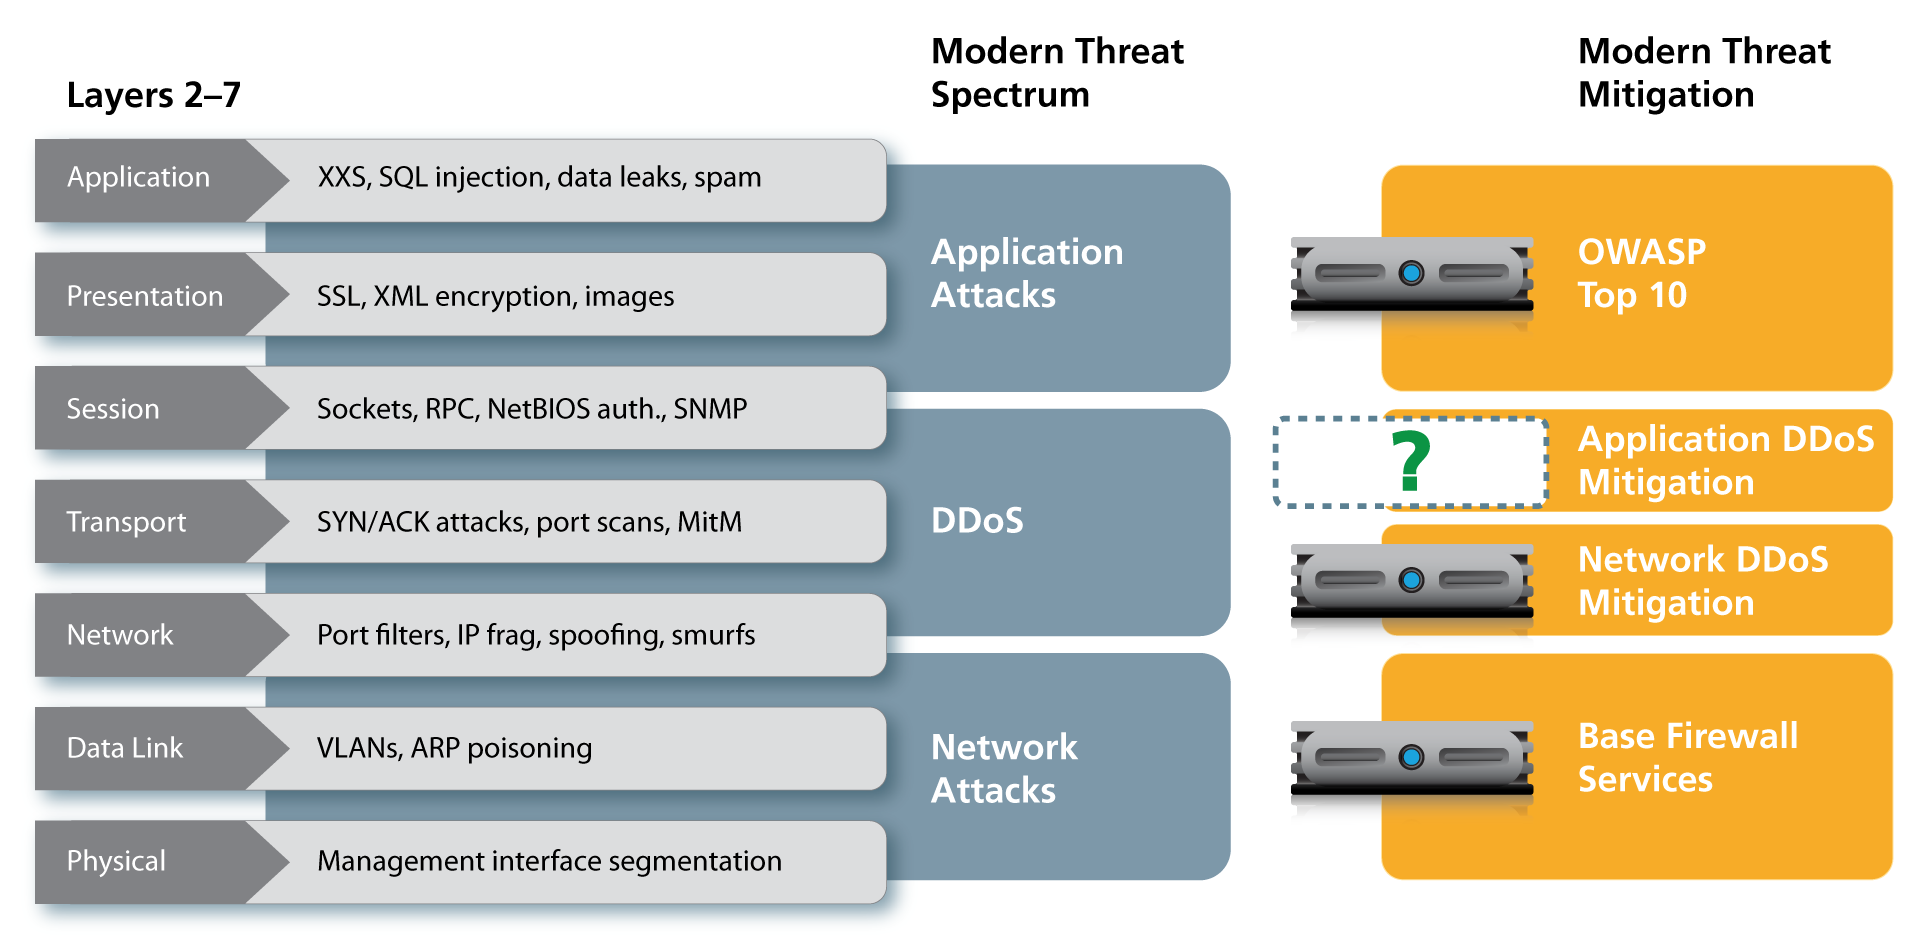
\includegraphics[width=450px]{./assets/img/osithreats.png}
	\caption{Possible threats at each OSI model layer and possible mitigation techniques.}
\end{figure}

Web threats can target any level of the OSI model in order to exploit different weaknesses or perform different types of attacks for various reasons (Figure \ref{fig:osithreats}).  Application attacks, which this research is focusing on, occur on the Application, Presentation, and partially the Session layers.  While several of these attacks can be mitigated by preventing the OWASP Top10 security flaws, it is only mitigation and there is always the possibility for a new attack variant to slip past.

Attacks will always prefer the most vulnerable target, the weakest link, and there is nothing more vulnerable than the public-facing application.  Studies have found that many of the existing techniques for handling these application layer attacks suffer from one or more of the following techniques:

\begin{itemize}
	\item Inherent limitations
	\item Incomplete implementations
	\item Complex frameworks
	\item Runtime overheads
	\item Intensive manual work requirements
	\item False positives and false negatives
\end{itemize}
% a survey on web application vulnerabilities
This means that despite the fact that these attacks are considered easy to mitigate, the existing solutions are not completely adequate for defending against some of the most common web attacks.  In order to solve this problem new methods of detection and prevention need to explored and older conventional methods need to be improved.

\section{SQL Injection}
Structured Query Language or SQL or short is the most dominant language for interacting with relational databases in recent years.  A SQL injection is an attack where through various means arbitrary unauthorized SQL code is ran on the database.  When one of the primary reasons behind performing these attacks is to gather confidential data this is an obvious means of acquiring the information.% a survey on web...
There are four common methods of injecting the SQL commands into the application:

\begin{itemize}
	\item Injection through user input
	\item Injection through cookies
	\item Injection through server variables
	\item Second-order injections
\end{itemize}

Injection through user input is the simpliest method, where the malicious user simply enters the arbitrary SQL code into any field that has some interaction with the database.  Injection through cookies involves applications that read from the cookie's fields to restore the users state, this information can be modified to contain SQL code to be read on returning to the website.  Injection through server variables such as PHP session variables, or other environment variables are used in a similar manner to cookies by applications and can be exploited in a similar fashion.  Lastly, second-order injections are some of the hardest to detect because they involve an attack that occurs later on after the data is entered. % A classification of SQL injection attacks

The impact and purpose of SQL injections can be broken down into four main categories.  First, \textbf{confidentiality} is lost, database that hold sensitive information which may be financial or identifiable is compromised and can now be considered public knowledge. % talk about PCI compliance
Secondly, in addition to the data being potentially leaked it now also has its \textbf{integrity} compromised as the malicious user can make any modification he wants to the data.  \textbf{Authentication} and \textbf{authorization} of the application is also broken, it is now possible to log in as any user with any access level, removing the need for passwords and bypassing any safe guards.

While SQL injections are commonly used to retrieve the information from a database, there are much more nefarious things that can be done with it.  For example, previous wide-scale botnet attacks have used SQL injections mimicing as Google queries to facilitate malicious drive-by-download attacks on websites to spread malware.  % a survey on web... 
% get some sources on major data breaches.

\subsection{SQL Injection Types}

Often times many of these injection types are combined together and are not absolute, but the techniques can be classified under the six following categories.

\textbf{Tautology} attacks are designed to typically bypass authentication, identify injectable parameters or extract data.  It is typically done by using conditional SQL statements to evaluate to true in the WHERE portion of the query.  This will result in the query evaluating to true for every single row in the table and will often return all of them depending on how the application and the injection query is designed. For example the 1=1 portion of the following query will always evaluate to true:

\code{SELECT accounts FROM users WHERE login=’’ or 1=1 -- AND pass=’’ AND pin=}

A \textbf{malformed} or invalid query are often performed to gather information about the underlying database or applications structure to design more targetted queries.  This is due to the common mistake of having overly descriptive errors that reveal information that is very useful to an attacker. This can reveal information ranging from the DBMS used to the names of columns or tables.  The following example forces a conversion error:

\code{SELECT accounts FROM users WHERE login=’’ AND pass=’’ AND pin= convert (int,(select top 1 name from sysobjects where xtype=’u’))}

A third type of SQL injection exploits the \textbf{union} keyword which is used to combine rows of multiple tables.  This would often be used for extracting data as you can combine the data of another table which you only know a limited amount of information but is what you are interested in, with another table that is easily exploitable.  The following example combines the credit card information from another table with a null table, returning only the credit information which we are interested in:

\code{SELECT accounts FROM users WHERE login=’’ UNION SELECT cardNo from CreditCards where acctNo=10032 -- AND pass=’’ AND pin=}

\textbf{Piggy-backed} queries are where additional queries are added onto an existing query, this is the technique many people who have heard about when learning about SQL injections because it involves ending the current query and starting another.  This is typically done in the following syntax:
\code{; < Piggy-Backed Query > --} The semi-colon signifies the end of the current query, a new query is added, and then the remainder of the query is commented out, here is an example:

\code{SELECT accounts FROM users WHERE login=’doe’ AND pass=’’; drop table users -- ’ AND pin=123}

\textbf{Stored procedures} are typically designed to do something much greater than just extract data and instead do something much worse such as escalating themselves in the database environment or denying service.  Often times developers think that using embedded procedures makes their code protected from injections as all of the queries are within the database environment, but this is not the case. Given the following stored procedure to check our login credentials, we can inject \code{’ ; SHUTDOWN; --} and generate the following piggy-backed query.

\code{CREATE PROCEDURE DBO.isAuthenticated @userName varchar2, @pass varchar2, @pin int\\
AS\\
	EXEC("SELECT accounts FROM users\\
	WHERE login=’" +@userName+ "’ and pass=’" +@password+ "’ and pin=" +@pin);\\
GO}

\code{SELECT accounts FROM users WHERE login=’doe’ AND pass=’ ’; SHUTDOWN; -- AND pin=}

The last category are \textbf{inference} attacks, these are used where malformed queries cannot be used to provide vital information to construct attacks.  Instead, injections are preformed and the website is monitored for changes or a response, this information is used to deduce vulnerable parameters and information on the values in the database.  There are two types of inference attacks, \emph{blind injections} and \emph{timing attacks}. Blind injections are posing simple true or false queries to the database, if the query evaluates to true then nothing will change, but a false evaluation will typically differ in some way.  For example, the two following queries should both return an error if the input is handled properly, but if only the first one returns an error than the login parameter is vulnerable:  

\code{SELECT accounts FROM users WHERE login=’legalUser’ and 1=0 -- ’ AND pass=’’ AND pin=0\\
SELECT accounts FROM users WHERE login=’legalUser’ and 1=1 -- ’ AND pass=’’ AND pin=0}

Timing attacks make use of the \code{WAITFOR} keyword to note the increase or decrease in the response time instead of an error message.  The following example is trying to extract table names by using a binary search method, if there is a delay in the response then the attacker knows how to adjust his search.

\code{SELECT accounts FROM users WHERE login=’legalUser’ and ASCII(SUBSTRING((select top 1 name from sysobjects),1,1)) > X WAITFOR 5 -- ’ AND pass=’’ AND pin=0}

It is also important to note that any of these attacks and the future discussed attacks can also obscure their presence by using alternative encodings for the text that is entered, for example input can be converted to unicode or hexadecimal.
% A classification of SQL-injection attacks

\section{Cross-Site Scripting}

Cross-site scripting attacks or XSS for short are similar to SQL injections in that the arbitrary code is injected from user inputs but instead of influencing the database it will leverage the facing code of the web application, more often the HTML or Javascript.  XSS attacks can be used for a variety of purposes, to redirecting users to other websites or just simply changing the look of the website.  In the worst case, XSS attacks can be used to hijack users sessions to collect information from the user.

It is hard to pinpoint the level of impact of a XSS attack because it all depends on what it is being used for.  XSS attacks, unlike SQL injections can be just a minor nuisence or can be just as severe and collect sensitive information.  Often times instead of a XSS attack being used alone, it is instead used as part of a larger scheme to send a user to another attack website where a phishing attack or something of similar nature lies.
% a survey on web...
%xssdm...

\subsection{Types of Cross-Site Scripting Attacks}

The first type of XSS attack is called a \textbf{stored} or \textbf{persistent} attack.  These are attacks that are permanently stored in a database, whenever a user access the page that retrieves the information from the database they're browser runs the attack. A simple example is just inserting typical HTML code into a comment field.

The second type of XSS attack is referred to as a \textbf{reflected} attack.  Instead of the result being stored in the remote-server they instead originate from another source, sometimes an email link or another website, upon clicking the link the code runs as the browser considers it from a safe source.  These attacks are non persistent because you would have to click the original link again for the attack to run as it is not tied to the page like in a stored attack.
%OWASP XSS

The final type of XSS attack is a newer distinction for XSS attacks called a \textbf{Document Object Model (DOM) based} attack.  In this variant, the attack is ran through modifying the actual document model through javascript's document object.  What seperates this attack from a stored or reflected attack is the original page does not change, but instead of users actions will result in a different result because their environment has been modified.
%owasp DOM XSS

\section{Remote File Inclusion}

The final web-threat that will be examined in this research is remote file inclusion also known as RFI.  Put simply, it is using the vulnerabilities of the application to include remote files which may include arbitrary code of any language.  The most common example is abusing PHP's include() command to get some PHP code to run on the remote server.  RFI attacks allow for code execution on the remote server and client-side, denial of service attacks due to remote shells and data extraction.
% OWASP RFI

Whle there are not any predefined variants for RFI attacks, for the purposes of this research RFI attacks will be divided into the following three categories:

\begin{itemize}
	\item Only parameters with URLs
	\item Only paramters with PHP commands
	\item Parameters with URLs and PHP commands
\end{itemize}
